%   File: Babyboot.tex
% Author: Adam Leeper (with modifications by Paul Mitiguy)
%------------------------------------------------------------------------------
%\\[0.45pc]
\providecommand{\isolatedBuild}[1]{#1}% Fallback definition to build normally.
\isolatedBuild{
  \documentclass[11pt,letterpaper]{book}
  %\documentclass[11pt,letterpaper]{book}

% aleeper: I think these are needed for Paul's macros?
\usepackage{epsfig}
\usepackage{epstopdf}

%\makeatletter
%\typeout{The import path is \import@path}
%\makeatother

\usepackage{import}

\subimport{./}{packagesMitiguy.sty}
\subimport{./}{macrosMitiguy.tex}
\subimport{./}{PageStylesMitiguy.tex}
\subimport{./}{macrosLeeper.tex}
   % Found via TEXINPUTS environment variable.
  \isolatedBuildHeader{Angular Acceleration}
                      {Angular Acceleration of a Babyboot Pendulum}
}
%%%
%%%
%%%
\begin{minipage}{0.55\textwidth}
A babyboot pendulum (as shown in class) is pictured at right,
consisting of a rod \basis{A} and rectangular plate \basis{B}.
Assume the support structure is a Newtonian reference frame \basis{N}.
Sets of right-handed  orthogonal unit vectors are fixed in each frame as shown,
and angles $\theta$ and $\phi$ are indicated on the figure.
\\[0.5pc]
To clarify the figure,
$\theta$ is the angle between \uvecz{n} and \uvecz{a},
and $\phi$ is the angle between \uvecx{a} and \uvecx{b}.
%\\[0.5pc]
%Clearly \textbf{explain} why we can say $\angvel{A}{N} = + ~\thetadot~\uvecx{a}$.
%\\[0.25pc]
%Clearly \textbf{explain} why we can say $\angvel{B}{A} = + ~\phidot~\uvecz{a}$.
%\\[0.25pc]
%(I gave them to you so that you can do the rest of the problem, but you need to
%\textbf{convince me} that you could come up with those expressions on your own.)
%\\[6.0pc]
\\[0.0pc]
\begin{itemize}
\item Form \angvel{A}{N} and \angvel{B}{A} by inspection.
\item Use the \textbf{definition} to \textbf{compute} \basis{B}'s angular acceleration in \basis{N} in terms of symbols and unit-vectors.
\end{itemize}
\vspace{12.pc}
\end{minipage}
\hfill
\begin{minipage}{0.38\textwidth}
\flushright
\includegraphics[width=0.96\columnwidth]{babyboot2.png}
\end{minipage}
\isolatedBuildFooter